\documentclass[8pt]{beamer}

\mode<presentation> {
\usetheme{Madrid}
\setbeamertemplate{footline}[page number]
}

\usepackage{graphicx} % Allows including images
\usepackage{booktabs} % Allows the use of \toprule, \midrule and \bottomrule in tables
\usepackage{tabularx}  % for 'tabularx' environment and 'X' column type
\usepackage{ragged2e}  % for '\RaggedRight' macro (allows hyphenation)
\usepackage{grffile}
\newcolumntype{Y}{>{\RaggedRight\arraybackslash}X} 

\usepackage{amsfonts}
%\usepackage{tikz}
%\def\checkmark{\tikz\fill[scale=0.4](0,.35) -- (.25,0) -- (1,.7) -- (.25,.15) -- cycle;} 


\setcounter{figure}{0}

\title[Energy Efficient Vehicle Control]{Real World Optimization of Energy Efficient Vehicle Control}
\subtitle[Current State]{}
\author{Bastian Lang} % Your name
\institute[BRSU] % Your institution as it will appear on the bottom of every slide, may be shorthand to save space
{
Bonn-Rhein-Sieg University of Applied Science \\ % Your institution for the title page
}
\date{\today} 
%\titlegraphic{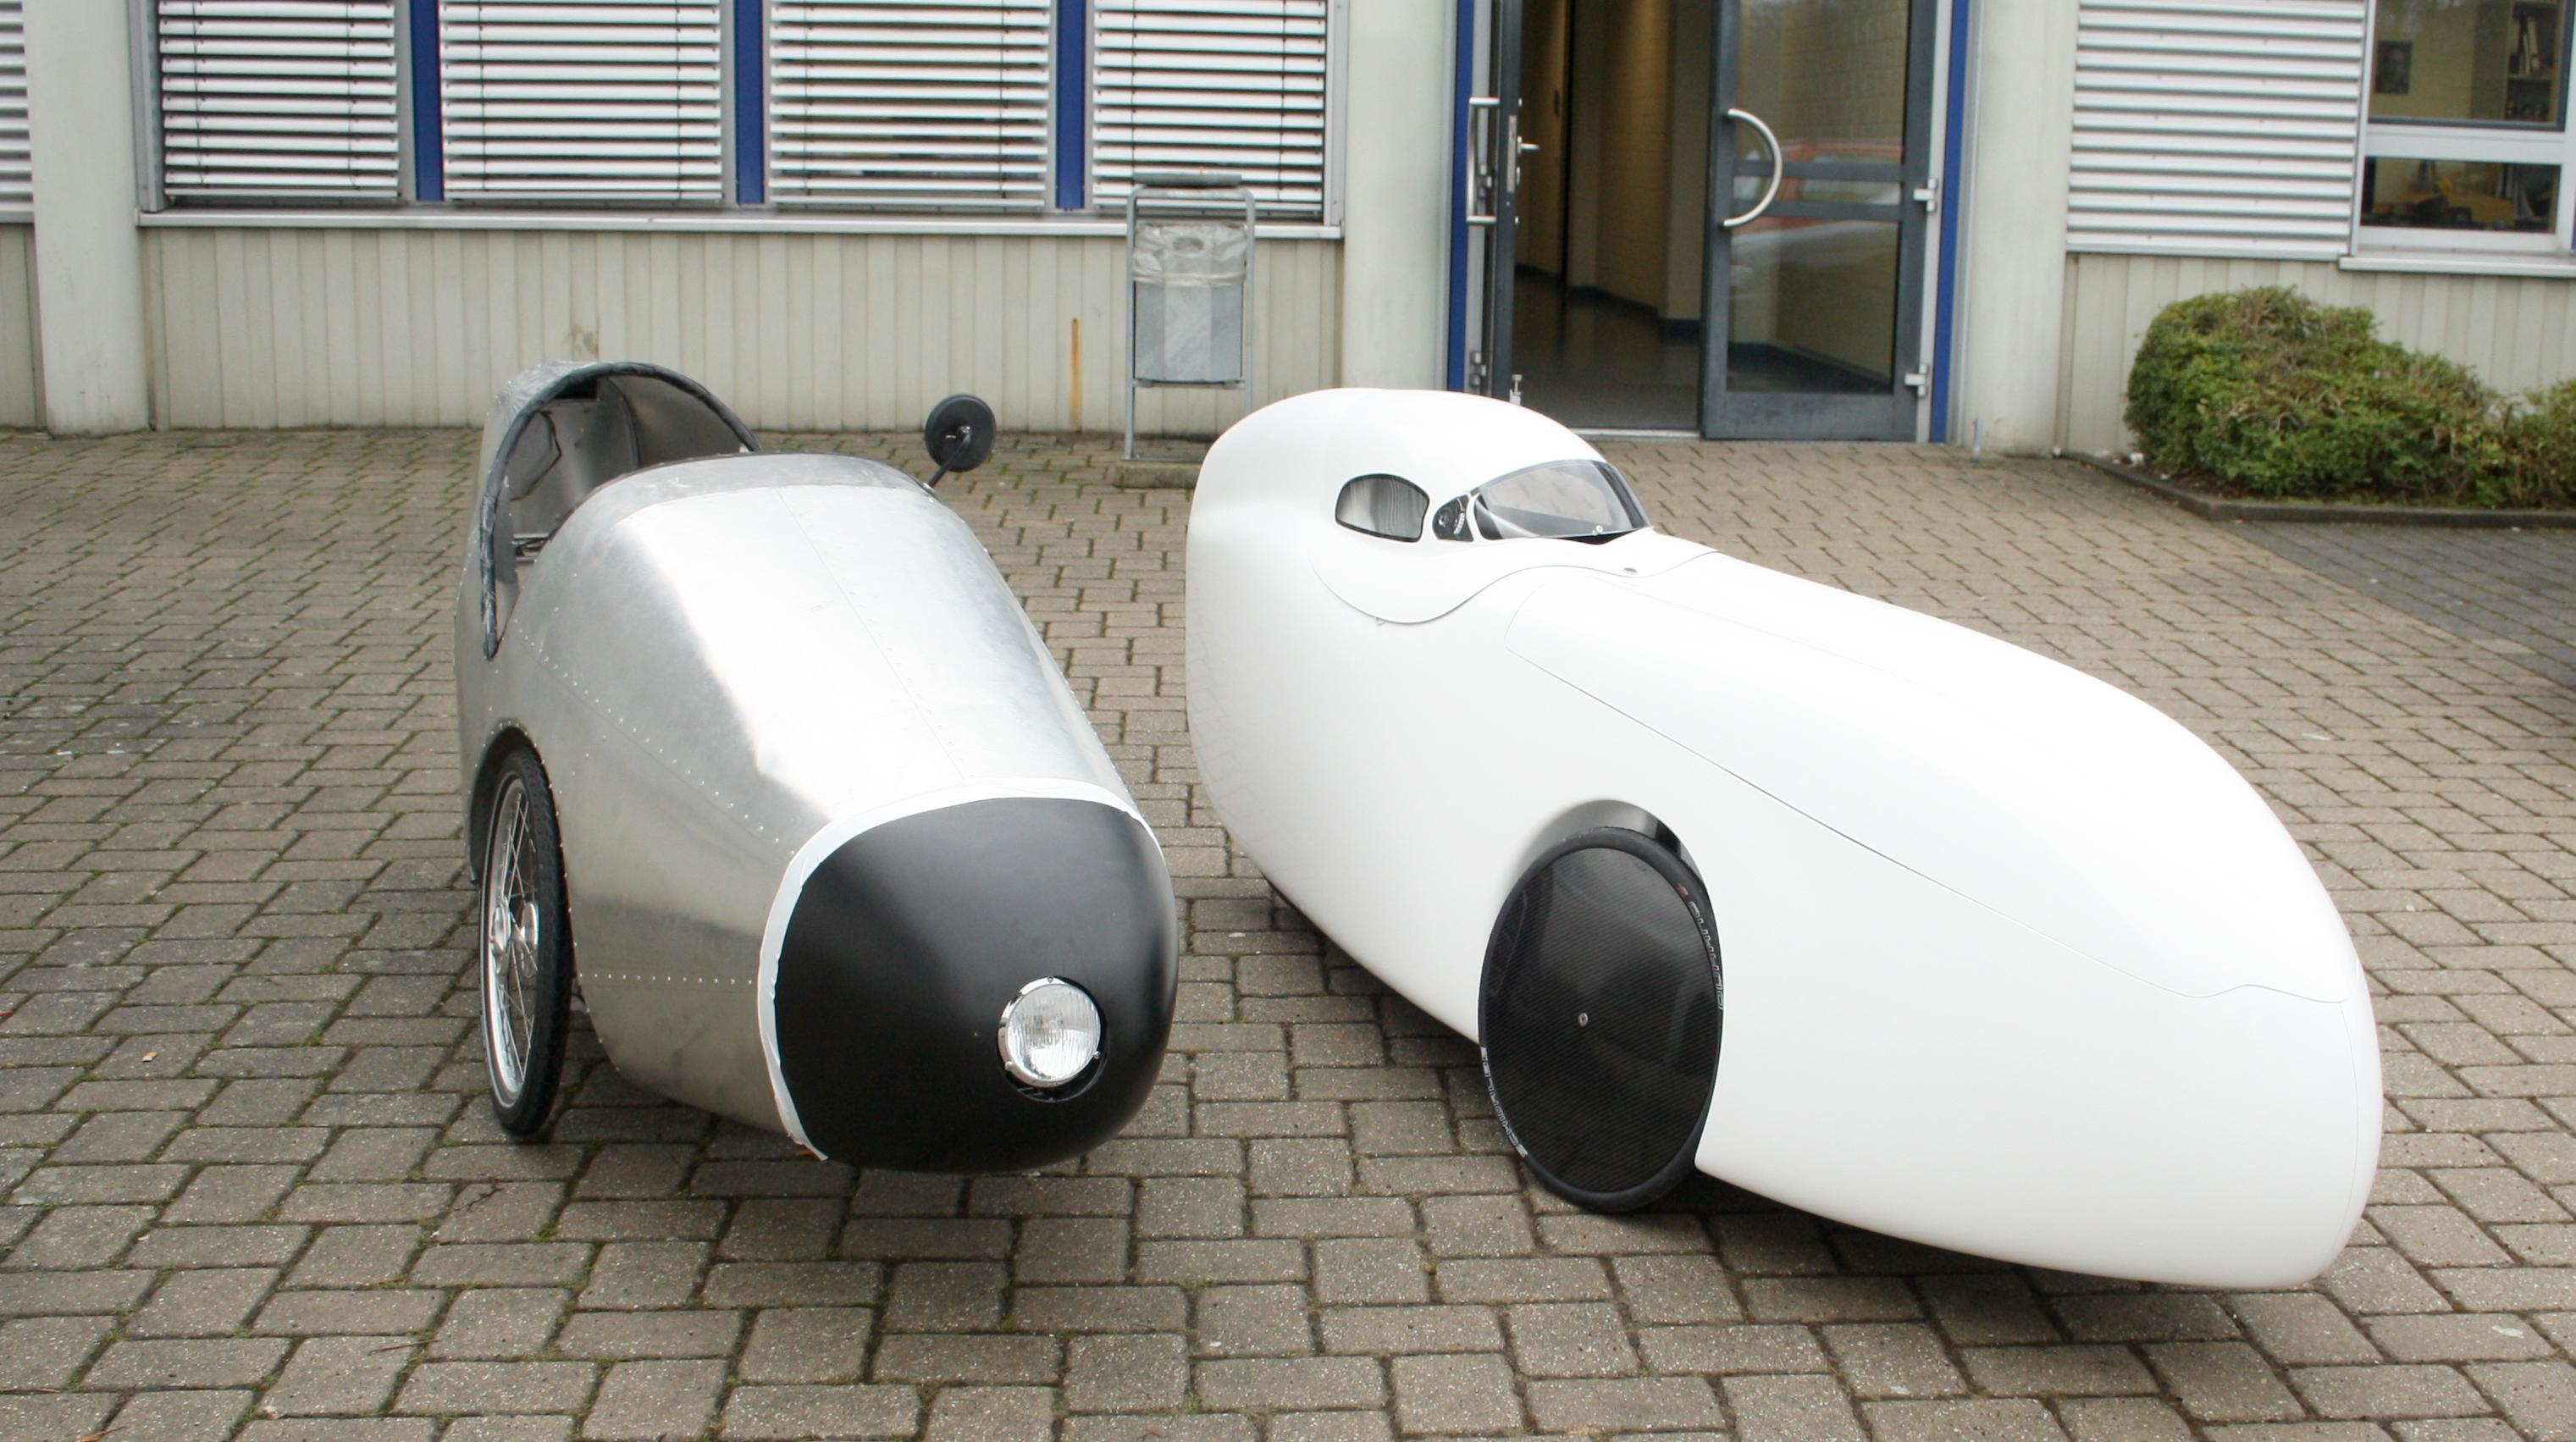
\includegraphics[width=6cm]{images/stella}}
\begin{document}

\listoffigures

\begin{frame}
	\titlepage
\end{frame}

\begin{frame}
	\frametitle{Content}
	\tableofcontents[hideallsubsections]
\end{frame}

\section{Project Description}
\begin{frame}
	\frametitle{Project Description}
	\framesubtitle{Project Description}
	\begin{block}{What is the project about?}
		Creating Energy Efficient Vehicle Controller  
	\end{block}	
	\pause	
	\begin{block}{What ML technologies are being used?}
		ANNs evolved using NEAT
	\end{block}
	\pause
	\begin{block}{What is the project based on?}	
		Paper showing ANNs can compete with state-of-the-art approaches (\cite{gaier2014evolving})
	\end{block}
\end{frame}

\begin{frame}
	\frametitle{Project Description}
	\framesubtitle{Task Overview}
	\begin{block}{Minimum}
	\begin{itemize}[<+->]
		\item Evolve Energy Efficient Controller with Simple Model
		\item Evaluate in Reality 
		\item Compare Simulation vs Reality
	\end{itemize}
	\end{block}	
	\pause
	
	\begin{block}{Expected}
	\begin{itemize}[<+->]
		\item Create Data Driven Model 
		\item Evolve Energy Efficient Controller with DD Model
		\item Evaluate in Reality
		\item Compare Solutions		
	\end{itemize}
	\end{block}	
	\pause
	
	\begin{block}{Maximum}
	\begin{itemize}[<+->]
		\item Use Multi-Objective Approach (i.e. Surrogate Modelling)
	\end{itemize}
	\end{block}
	
\end{frame}



\section{The Simple Model}
\begin{frame}
	\frametitle{Content}
	\tableofcontents[currentsection, hideothersubsections]
\end{frame}
\begin{frame}
	\frametitle{Simple Vehicle Model}
	\begin{block}{Time Based Model}	
	\[
	\frac{ds}{dt} = \left(
			\begin{array}{ll}
			t' \\
			x' \\
			v' \\
			W'
			\end{array}
		\right)
		= \left(
			\begin{array}{ll}
			1 \\
			v \\
			\frac{F(x,v)}{m} \\
			F_u * v
			\end{array}
		\right)
	\]
	
	Where\\
	\begin{itemize}
		\item $F_U$: Force at wheel due to control command
		\item $F(x,v)$: $F_U$ - some drag
	\end{itemize}
	\end{block}

\end{frame}

\begin{frame}
	\frametitle{Simple Vehicle Model}
	TODO: Visualizations of Simulations
\end{frame}


\section{NEAT with Simple Model}
\begin{frame}
	\frametitle{Content}
	\tableofcontents[currentsection, hideothersubsections]
\end{frame}

\begin{frame}
	\frametitle{NEAT with Simple Model}
	\framesubtitle{NEAT}
	\begin{block}{Parameters}
		\begin{itemize}
			\item Population size: 60
			\item Maximum Generations: 40
			\item Speciation algorithm: k-means
			\item Number of Species: 3
			\item Drop-off rate: 25
			\item Dataset of 30/5 tracks (Training/Test)
		\end{itemize}
	\end{block}
	TODO: Plots of some tracks
\end{frame}

\begin{frame}
	\frametitle{NEAT with Simple Model}
	\framesubtitle{Evaluating Fitness}
	\begin{block}{On Set of Tracks}
		\begin{itemize}
			\item Weighted Sum of Single Track Fitnesses
		\end{itemize}
	\end{block}
	\pause
	\begin{block}{On Single Track}
		\begin{itemize}		
			\item Fitness: Saved Energy - Time Penalty
			\item Saved Energy: Maximum Energy Consumption - Actual Energy Consumption
			\item Time Penalty: \[\left\{ 
				\begin{array}{ll}
					0  & \mbox{if } neededTime \leq desiredTime \\
					(neededTime - desiredTime)^2 & \mbox{else } 
				\end{array}			
			\right. \]			
		\end{itemize}
	\end{block}	
\end{frame}

\begin{frame}
	\frametitle{NEAT with the Simple Model}
	\framesubtitle{Results}
	\begin{itemize}
		\item Average Best Fitness
		\item Average Nr Generations
	\end{itemize}
\end{frame}

\begin{frame}
	\frametitle{NEAT with the Simple Model}
	\framesubtitle{Simulations}
\end{frame}


\section{Control Program for Velomobile}
\begin{frame}
	\frametitle{Content}
	\tableofcontents[currentsection, hideothersubsections]
\end{frame}

\subsection{Given Hardware/Software}
\begin{frame}
	\frametitle{Control Program}
	\framesubtitle{Given}
	\begin{block}{Hardware}
		\begin{itemize}
			\item Velomobile
			\item Electric Motor (Vivax-Assist)
			\item Speed Controller (MasterSPIN 75 Pro OPTO)
			\item Brake Sensor
			\item Hall Sensor
			\item Power Sensor
			\item Simple Button
		\end{itemize}
	\end{block}	
	\pause
	\begin{block}{Software}
		\begin{itemize}
			\item Run motor on constant speed
			\item Read brake sensor
			\item Read hall sensor
			\item Shuts off above 25km/h
			\item Shuts off on brake activation
			\item Shuts off on button press
		\end{itemize}
	\end{block}		
\end{frame}

\subsection{Problems}
\begin{frame}
	\frametitle{Problems}
	\framesubtitle{Reading Hall Sensor}
	\begin{block}{Why a Problem?}
	\begin{itemize}
		\item Needed for velocity data
		\item Python-code to read sensor
		\item C-code to control motor
		\item Not implemented
	\end{itemize}		
	\end{block}
	\pause
	\begin{block}{Solution}
		\begin{itemize}[<+->]
			\item Write/read file in python/C $\rightarrow$ Synchronization
			\item Write/Read output stream $\rightarrow$ Python script needs to call C script and resets state
			\item Use socket communication
		\end{itemize}
	\end{block}
\end{frame}

\begin{frame}
	\frametitle{Problems}
	\framesubtitle{Speed Adaptation}
	\begin{block}{Why a Problem?}
		\begin{itemize}
			\item Needed for collecting data
			\item Not implemented
		\end{itemize}
	\end{block}
	\begin{block}{Solution}
		\begin{itemize}
			\item Increase speed on button click
			\item Shut motor off on brake activation only
		\end{itemize}
	\end{block}	
\end{frame}

\begin{frame}
	\frametitle{Problems}
	\framesubtitle{No Motor Reaction}
	\begin{block}{Why a Problem?}
		\begin{itemize}
			\item Cannot drive vehicle
		\end{itemize}
	\end{block}
	\begin{block}{Solution}
		\begin{itemize}
			\item (Hardware-)Debug with working initial code
			\item Only send signal on change
			\item Range [7,19] instead of [0,100]
		\end{itemize}
	\end{block}	
\end{frame}

\begin{frame}
	\frametitle{Problems}
	\framesubtitle{Huge Numbers in Log}
	\begin{block}{Why a Problem?}
		\begin{itemize}
			\item Obviously wrong data gets logged
			\item No synchronization during data access
		\end{itemize}
	\end{block}
	\pause
	\begin{block}{Solution}
		\begin{itemize}[<+->]
			\item Synchronize using mutexes $\rightarrow$ Still huge values
			\item Remove all possible multi-threading $\rightarrow$ Hall Sensor
			\item Rewrite in Python $\rightarrow$ Files empty, occasional restarts
		\end{itemize}
	\end{block}	
	\pause
	\begin{block}{Open Approaches}
		\begin{itemize}
			\item Use C-code with wiringPi synchronization mechanism
		\end{itemize}
	\end{block}
\end{frame}

\subsection{Control Program(s)}
\begin{frame}
	\frametitle{Software Architecture}
	TODO: Diagram
\end{frame}



\section{Open Tasks}
\begin{frame}
	\frametitle{Content}
	\tableofcontents[currentsection, hideothersubsections]
\end{frame}

\begin{frame}
	\frametitle{Open Tasks}
	\begin{block}{}
		\begin{itemize}
			\item Fix Logging
			\item Evaluate Solutions Simple Model
			\item Collect Data
			\item Learn Model
			\item NEAT on DD Model
			\item Evaluate Solutions DD Model
		\end{itemize}
	\end{block}
\end{frame}

\begin{frame}[allowframebreaks]
\frametitle{Sources}
\bibliographystyle{apalike}
\bibliography{Biblio-Database}

\end{frame}


\end{document} 